\documentclass{beamer}
\usepackage[T1]{fontenc}
\usepackage[utf8]{inputenc}
\usepackage{lmodern}

\usepackage{graphicx}
\graphicspath{{data/}}

\title{ROS : Robot Operating System}
\author{Weipeng He \\ \texttt{2he@informatik.uni-hamburg.de}}
\date{5 November, 2012}

\begin{document}

\frame{\titlepage}

\begin{frame}
\frametitle{Outline}
\tableofcontents
\end{frame}

\section{Introduction}
\begin{frame}
\frametitle{Introduction}
\framesubtitle{What is ROS?}
\begin{center}
  
\includegraphics[width=.4\textwidth]{ros_org}
\end{center}
\begin{itemize}
  \item ROS is Robot Operating System.
  \item ROS is an open-source, meta-operating system for robots.
  \item It provides the services including hardware abstraction, low-level device control, implementation of commonly-used functionality, message-passing between processes, and package management.
  \item It also provides tools and libraries for obtaining, building, writing, and running code across multiple computers.
\end{itemize}
\end{frame}

\begin{frame}
\frametitle{Introduction}
\framesubtitle{History}
\begin{itemize}
  \item ROS was originally developed in 2007 under the name switchyard by the Stanford Artificial Intelligence Laboratory in support of the Stanford AI Robot (STAIR) project.
  \item From 2008, development continues primarily at Willow Garage, with more than twenty institutions collaborating in a federated development model.
  \item April 23, 2012 the latest stable release : Fuerte.
  \item Now, ROS works on different operating systems (Linux, Mac OS, Windows, FreeBSD, etc.).
  \item ROS can be developed in C++, Python and Lisp.
  \item More than 80 robots(PR2, Care-O-bot 3, iRobot Create, Aldebaran Nao, etc.) are listed as supported by ROS.
\end{itemize}
\end{frame}

\section{Motivation}
\begin{frame}
\frametitle{Motivation}
\framesubtitle{Some facts about research in robotics}

\begin{itemize}
  \item It's difficult to reproduce the experiment results from other's publication.
  \item Researchers use different robots. The hardware are very different.
  \item Sometimes, researchers from different groups just do the same coding work.
  \item What if they have a platform that they can use to collaborate?
\end{itemize}
\end{frame}

\begin{frame}
\frametitle{Motivation}
\framesubtitle{Pose tracking}

\begin{itemize}
  \item Suppose I need to develop a program to track the pose of an robot arm.
  \begin{center}
    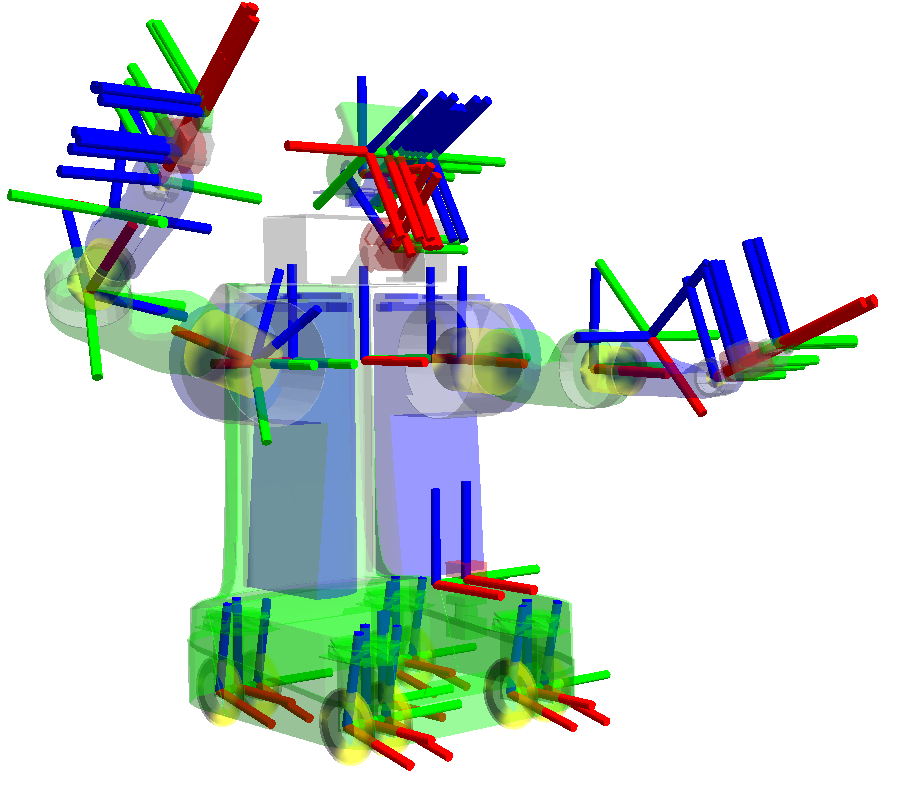
\includegraphics[width=.4\textwidth]{tf_pr2}
  \end{center}
  \item tf in ROS : keep track of multiple coordinate frames over time.
\end{itemize}
\end{frame}

\begin{frame}
\frametitle{Motivation}
\framesubtitle{We can use ROS}

\begin{itemize}
  \item The primary goal of ROS is to support code reuse in robotics research and development.
  \\ ~  
  \item Well-designed software structure.
  \item Numerous libraries and drivers.
  \item Utilities which assist development.
  \item Community support.
\end{itemize}
\end{frame}

\section{Software Structure}
\begin{frame}
\frametitle{Software Structure}
\framesubtitle{ROS Computation Graph}

\begin{itemize}
  \item The ROS runtime "graph" is a peer-to-peer network of processes using the ROS communication infrastructure.
\end{itemize}
\begin{center}
  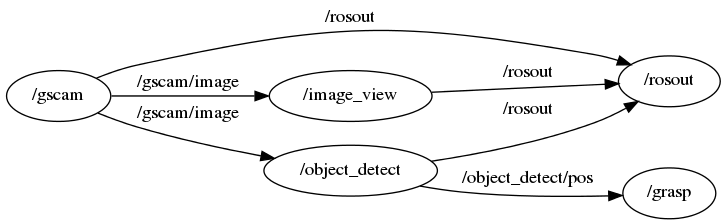
\includegraphics[width=\textwidth]{comp_graph}
\end{center}

\end{frame}

\begin{frame}
\frametitle{Software Structure}
\framesubtitle{Node and Master}

\begin{itemize}
  \item Nodes are processes that perform computation. 
  \item ROS is designed to be modular at a fine-grained scale. Robot control system will usually comprise many nodes.
  \item For example, one node controls a laser range-finder, one node controls the wheel motors, one node performs localization, one node performs path planning, one node provides a graphical view of the system, and so on.
  \item Nodes get to know each other via roscore (master).
\end{itemize}

\begin{center}
  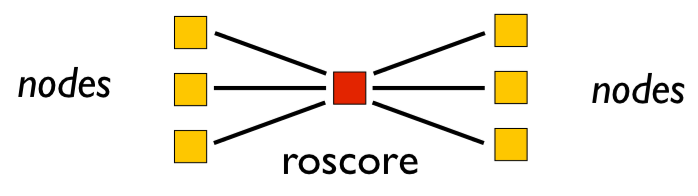
\includegraphics[width=.6\textwidth]{nodes}
\end{center}

\end{frame}

\begin{frame}
\frametitle{Software Structure}
\framesubtitle{Message}

\begin{itemize}
  \item Nodes communicate with each other by passing messages.
  \item A message is simply a data structure, comprising typed fields. 
  \item Standard primitive types (integer, floating point, boolean, etc.) are supported, as are arrays of primitive types. 
  \item Messages can include arbitrarily nested structures and arrays (much like C structs).
\end{itemize}
\end{frame}

\begin{frame}
\frametitle{Software Structure}
\framesubtitle{Message example}

\begin{itemize}
  \item sensor\_msg/Image
\end{itemize}

Header header \\
~  uint32 seq \\
~  time stamp \\
~  string frame\_id \\
uint32 height \\
uint32 width \\
string encoding \\
uint8 is\_bigendian \\
uint32 step \\
uint8[] data
\end{frame}

\begin{frame}
\frametitle{Software Structure}
\framesubtitle{Topic}

\begin{itemize}
  \item Topic is a mechanism to send messages from a node to one or more nodes.
  \item Follows a publisher-subscriber design pattern.
  \item Publisher is the node which send messages to the topic.
  \item Subscribers are the nodes which get called whenever a message is published.
  \item Example : Camera publishing images.
\end{itemize}

\begin{center}
  
\includegraphics[width=.6\textwidth]{topic}
\end{center}

\end{frame}

\begin{frame}
\frametitle{Software Structure}
\framesubtitle{Service}

\begin{itemize}
  \item Service is a mechanism for a node to send a request to another node and receive a response in return.
  \item Follows a request-response design pattern.
  \item A service is called with a request message, and in return, a response message is returned.
  \item Example : Request the camera to tilt.
\end{itemize}

\begin{center}
  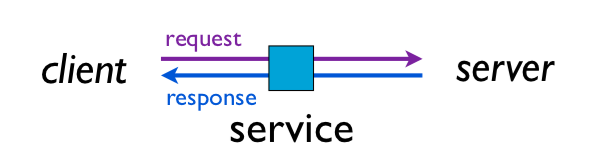
\includegraphics[width=.6\textwidth]{service}
\end{center}
\end{frame}

\begin{frame}
\frametitle{Software Structure}
\framesubtitle{File system Hierarchy}

\begin{itemize}
  \item Release : collection of stacks and packages.
  \begin{itemize}
    \item Fuerte
  \end{itemize}
  \item Stacks : a full application suite.
  \begin{itemize}
    \item geometry
  \end{itemize}
  \item Package : software to solve a specific task.
  \begin{itemize}
    \item tf
  \end{itemize}
  \item Node : an executable.
  \begin{itemize}
    \item tf\_echo
  \end{itemize}
\end{itemize}

\end{frame}

\section{Community}
\begin{frame}
\frametitle{Community}
\framesubtitle{Software Distribution}

\begin{itemize}
  \item ROS code is maintained in a decentralized federation of repositories.
  \begin{itemize}
    \item The core repository : ros-pkg;
    \item 94 repositories in other institutions;
    \item 14 personal repositories.
  \end{itemize}
  \item Easy to contribute.
  \begin{itemize}
    \item Host their code (and documents) in their own repository.
    \item SourceForge.net, Google Code and GitHub.
    \item Register at ros.org.
  \end{itemize}
  \item Easy to search software.
  \begin{itemize}
    \item Search across the federation of repositories is possible.
    \item ros.org keeps tracks of updates of all repositories and generates index.
    \item Documentation and tutorials are also updated automatically.
  \end{itemize}
\end{itemize}

\end{frame}

\begin{frame}
\frametitle{Community}

\begin{itemize}
  \item ROS Answers.
\end{itemize}
\begin{center}
  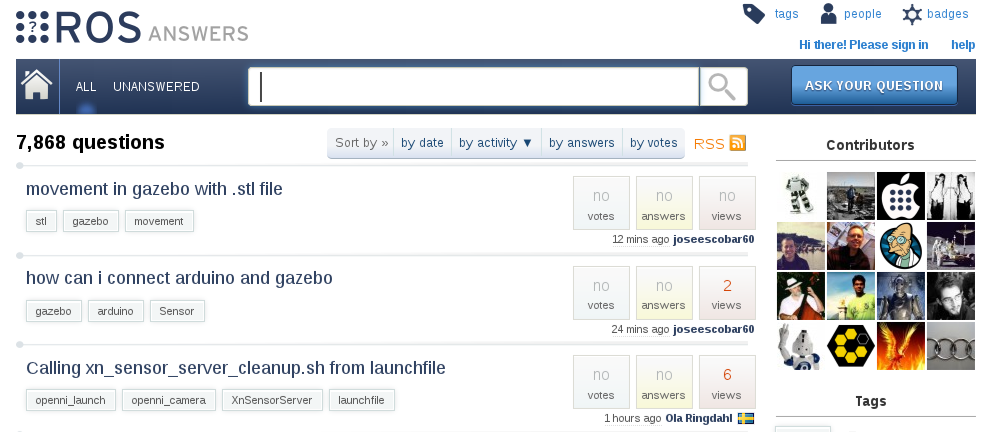
\includegraphics[width=\textwidth]{ros_answers}
\end{center}
\end{frame}

\section{Conclusion}
\begin{frame}
\frametitle{Conclusion}

\begin{itemize}
  \item ROS defines a standard for the communicate mechanisms and protocols between robot components.
  \item ROS provides libraries for various functions.
  \item ROS contains utility tools to help development.
  \item ROS promotes code sharing and reuse.
\end{itemize}

\end{frame}

\begin{frame}
\frametitle{Questions?}
Thanks!
\end{frame}


\end{document}
